\documentclass[12pt,twoside]{book}
% \usepackage{cite}
% \usepackage[pdftex]{graphicx}
% \usepackage{array}
\usepackage{amsmath}

% \usepackage{bm}
% \usepackage{stmaryrd}
% \usepackage[tight,footnotesize]{subfigure}

\DeclareMathOperator*{\argmax}{arg\,max}
\DeclareMathOperator*{\argmin}{arg\,min}

\newcommand{\meutitulo}{Aprendizado ativo ... }
\newcommand{\meunome}{Davi Pereira dos Santos}
\newcommand{\meuorientador}{Prof. Dr. Andr� Carlos Ponce de Leon Ferreira de Carvalho}
\newcommand{\minhadata}{Dezembro/2014}
\newcommand{\minhabolsa}{Trabalho realizado com o apoio da CAPES.}
\newcommand{\meugrau}{Doutor}

%portugues
\usepackage[ruled,linesnumbered,vlined]{algorithm2e}
\usepackage{fancyhdr}

\usepackage{ textcomp }

%\renewcommand{\listalgorithmcfname}{Lista de Algoritmos}%
%\renewcommand{\algorithmcfname}{Algoritmo}%
\usepackage[english,brazil]{babel}
\usepackage{subfigure}
%%\usepackage{epigraph}
%%\usepackage{endnotes}
%\renewcommand{\notesname}{Coment�rios}
\usepackage{natbib}
\usepackage{latexsym}
\usepackage{setspace}
\usepackage{xspace}
% \usepackage[nohyperlinks]
%%% referencias com p�gina \vref
\usepackage[brazil]{varioref}
\usepackage{indentfirst}
%%% figuras um ao lado do outro
\usepackage{subfigure}
%%% definir t�tulos de se��o
\usepackage[sf,sl,outermarks]{titlesec}
\titleformat{\section}{\color{black}\normalfont\Large\bfseries}{\color{darkgray}\thesection}{1em}{}
\titleformat{\subsection}{\color{black}\normalfont\bfseries}{\color{darkgray}\thesubsection}{1em}{}

%%% boxes
\usepackage{fancybox}
\usepackage{fancyvrb}
\usepackage[usenames,dvipsnames]{color}
%\usepackage[pdftex]{graphicx}
\usepackage{graphicx}
\usepackage[pdftex]{geometry}
  \geometry{a4paper,left=3cm,right=2cm,top=2.0cm,bottom=2cm,twoside}

%%% cria links no arquivo .pdf
%%% comentar as linhas na vers�o para impressao
\usepackage[pdftex,pdfpagelabels,pagebackref,pageanchor=false]{hyperref}

% % Para imprimir PDFs com offset
% \begin{document}
% \begin{figure} %[H]
%     \centering
%     \includegraphics[bb=640 0 0 850]{/home/davi/12.pdf}
% %     \caption{\textit{Generative ensembles}}
% %     \label{gen}
% \end{figure}
% \end{document}


\usepackage{pdfpages}
\usepackage{multirow}
\usepackage{makecell}
\hypersetup{
    pdftitle = {\meutitulo},
    pdfsubject = {},
    pdfkeywords = {},
    pdfauthor = {\meunome}
    }
\hypersetup{colorlinks=true,linkcolor=blue,citecolor=blue,hypertexnames=false}
% \usepackage[adobe-utopia]{mathdesign} %pacote texlive-fonts-extra no ubuntu
\usepackage{ae}
% \usepackage{bookman}
\usepackage[T1]{fontenc}
\usepackage{amsfonts}
\DeclareFixedFont{\numberfont}{T1}{phv}{bx}{n}{2cm}
\titleformat{\chapter}[display]
  {\normalfont\Large\sffamily
  }
  {%\titlerule[3pt]%
   \filright
   \rule[32pt]{.7\linewidth}{4pt}
   \hspace{-11pt}
   \shadowbox{
   \begin{minipage}{.18\linewidth}
     \begin{center}
       \textsc{\Large\chaptertitlename}\\
       \vspace{1ex}
       {\numberfont\color[gray]{0.5} \thechapter}\\
       \vspace{1ex}
     \end{center}
   \end{minipage}}
  }
  {0pt}
  {\filcenter
   \Huge
   }
  [\hfill\rule{.8\textwidth}{0.5pt}\\
     \vskip-1.8ex\hfill\rule{.7\textwidth}{3pt}]

\newcommand{\versal}[1]{{\noindent
    \setbox0\hbox{\largefont #1 }%
    \count0=\ht0                   % height of versal
    \count1=\baselineskip          % baselineskip
    \divide\count0 by \count1      % versal height/baselineskip
    \dimen1 = \count0\baselineskip % distance to drop versal
    \advance\count0 by 1\relax     % no of indented lines
    \dimen0=\wd0                   % width of versal
    \global\hangindent\dimen0      % set indentation distance
    \global\hangafter-\count0      % set no of indented lines
    \hskip-\dimen0\setbox0\hbox to\dimen0{\raise-\dimen1\box0\hss}%
    \dp0=0in\ht0=0in\box0}}

\definecolor{dark-green}{rgb}{0,0.5,0}
\newcommand{\X}{X\xspace}
\newcommand{\Y}{Y\xspace}
\newcommand{\xt}{\bm{x}_{(t)}\xspace}
\newcommand{\x}{\bm{x}\xspace}
\newcommand{\yt}{\bm{y}_{(t)}\xspace}
\newcommand{\y}{\bm{y}\xspace}
\newcommand{\pool}{reserva de exemplos\xspace}
\newcommand{\pools}{reservas de exemplos\xspace}
\newcommand{\U}{\mathcal{U}\xspace}
\newcommand{\Ut}{\U_{(t)}\xspace}
\newcommand{\Lt}{\mathcal{L}_{(t)}\xspace}
\newcommand{\tra}[2]{\underline{#1}\xspace\footnote{\textit{#2}\xspace}}
\newcommand{\blue}[1]{\textcolor{blue}{#1}\xspace}
\newcommand{\red}[1]{\textcolor{red}{#1}\xspace}
\newcommand{\green}[1]{\textcolor{dark-green}{#1}\xspace}
\newcommand{\esb}[1]{\blue{#1}\xspace}
\newcommand{\ano}[1]{\red{[$\star$ #1 $\star$]}\xspace}
\newcommand{\tar}[1]{\green{$\star$ #1}\xspace}
\newcommand{\versionspace}{espa�o de vers�es\xspace}

\newcommand{\ing}[2]{\emph{#1}\footnote{\textit{#2}}}
\newcommand{\novo}[1]{\emph{#1}}
\newcommand{\eer}{redu��o do erro esperado\xspace}
\newcommand{\Eer}{Redu��o do erro esperado\xspace}
\newcommand{\elms}{\textit{m�quinas extremas}\xspace}
\newcommand{\elm}{\textit{m�quina extrema}\xspace}
\newcommand{\svm}{m�quina de vetores de suporte\xspace}

\newcommand{\tarefa}[1] {\addcontentsline{toc}{section}{\tar{#1}}}







\newcommand{\emphFirst}[1] {\textbf{#1}}

\renewcommand{\reftextfacebefore}{}
\renewcommand{\reftextfaceafter}{}

\newcommand{\mx}{\hbox{\textbf{x}}\xspace}
\newcommand{\smx}{\hbox{{\scriptsize \textbf{x}}}\xspace}

\newcommand{\ranking}{\hbox{\textit{ranking}}\xspace}



% Backref com coloca��o de "Citado na p�gina..."
\renewcommand*{\backref}[1]{}
\renewcommand*{\backrefalt}[4]{
    \ifcase #1
        N�o citado no texto.
    \or
        Citado na p�gina~#2.
    \else
        Citado nas p�ginas #2.
    \fi
}

\renewcommand{\backreftwosep}{ e~}
\renewcommand{\backreflastsep}{, e~}


\hyphenation{su-per-vi-sio-na-dos}
\hyphenation{su-per-vi-sio-na-do}


\newcommand{\gnuplot}{\textbf{GnuPlot$^{TM}$}\xspace}
\newcommand{\tfidf}{\textit{tfidf}\xspace}
\newcommand{\tflinear}{\textit{tflinear}\xspace}




\newcommand{\smooth}{\emph{smooth}\xspace}

\newcommand{\stempl}{\textbf{stem.pl}\xspace}
\newcommand{\reportpl}{\textbf{report.pl}\xspace}
\newcommand{\predictpl}{\textbf{predict.pl}\xspace}
\newcommand{\stembase}{\textbf{stembase}\xspace}
\newcommand{\textbase}{\textbf{textbase}\xspace}
\newcommand{\stoplist}{\textbf{stoplist}\xspace}


\newcommand{\sone}{\texttt{\%one\%}\xspace}
\newcommand{\stwo}{\texttt{\%two\%}\xspace}
\newcommand{\sthree}{\texttt{\%three\%}\xspace}
\newcommand{\sglobal}{\texttt{\%global\%}\xspace}
\newcommand{\stm}{\textit{stemming}\xspace}
\newcommand{\stemming}{\textit{stemming}\xspace}
\newcommand{\gram}{\textit{gram}\xspace}
\newcommand{\grams}{\textit{grams}\xspace}

\newcommand{\stems}{\textit{stems}\xspace}
\newcommand{\stem}{\textit{stem}\xspace}
\newcommand{\pretext}{\textsc{PreTexT}\xspace}
\newcommand{\script}{\textit{script}\xspace}
\newcommand{\scripts}{\textit{scripts}\xspace}
\newcommand{\stoplists}{\textit{stoplists}\xspace}
\newcommand{\stopfile}{\textit{stopfile}\xspace}
\newcommand{\stopfiles}{\textit{stopfiles}\xspace}
\newcommand{\stopword}{\textit{stopword}\xspace}
\newcommand{\stopwords}{\textit{stopwords}\xspace}


% experimentos
\newcommand{\news}{{\sc news}\xspace}
\newcommand{\course}{{\sc course}\xspace}
\newcommand{\lnai}{{\sc lnai}\xspace}
\newcommand{\ccourse}{{\tt course}\xspace}
\newcommand{\cncourse}{{\tt non-course}\xspace}
\newcommand{\sci}{{\tt sci}\xspace}
\newcommand{\talk}{{\tt talk}\xspace}
\newcommand{\texto}{\textsc{texto}\xspace}
\newcommand{\links}{\textsc{links}\xspace}

\newcommand{\cbr}{\textsc{cbr}\xspace}
\newcommand{\ilp}{\textsc{ilp}\xspace}





\newcommand{\kmeanski}
  {$k$-{\it means}$_{ki}$\xspace}

\newcommand{\kmeans}
  {$k$-me\-ans\xspace}


\newcommand{\clustering}
  {\textit{clustering}\xspace}



\newcommand{\kparticoes}
  {$k$-parti��es\xspace}

\newcommand{\coboosting}
  {\textsc{CO-BOOSTING}\xspace}

\newcommand{\boosting}
  {{\em Boosting}\xspace}


\newcommand{\bagging}
  {{\em Bagging}\xspace}

\newcommand{\naivebayes}
  {\emph{Naive Bayes}\xspace}

\newcommand{\bayes}
  {{\em Bayes}\xspace}

\newcommand{\framework}
  {\textsc{framework}\xspace}


% bullet
\newcommand{\bb}
  {\ensuremath{\bullet}}

% neck
\newcommand{\neck}
  {{\texttt{\bf\ :-\ }}}

% circ
\newcommand{\cc}
  {\ensuremath{\circ}}

% diamond
\newcommand{\dd}
  {\ensuremath{\diamond}}

% MLC++
\newcommand{\mlc}
  {\ensuremath{\mathcal{MLC\hspace{-.05em}\raisebox{.4ex}{\tiny\bf ++}}}\xspace}

% MySQL
\newcommand{\mysql}
%  {{\sc \smaller MySQL}\xspace}
  {\ensuremath{\mathcal{M}{\sf y}\mathcal{SQL}}\xspace}

% C++
\newcommand{\cplusplus}
  {\ensuremath{\mathcal{C\hspace{-.05em}\raisebox{.4ex}{\tiny\bf ++}}}\xspace}

% C++
\newcommand{\cpp}
  {\cplusplus}

% CI
\newcommand{\ci}
  {\ensuremath{\mathcal{CI}}\xspace}
%  {{\sc ci}\xspace}

% ID3
\newcommand{\idtree}
%  {{\sc id\relsize{-2}3}\xspace}
  {\ensuremath{\mathcal{ID}3}\xspace}

% GID3*
\newcommand{\gidtree}
  {{\sc gid\relsize{-2}3*}\xspace}

% Skicat
\newcommand{\skicat}
  {{\sc \smaller Skicat}\xspace}

% PBM
%\newcommand{\pbm}
 % {{\sc \smaller pbm}\xspace}

%PBM
\newcommand{\pbm}
   {\ensuremath{\mathcal{PBM}}\xspace}

% C4.5
\newcommand{\cfourfive}
%  {{\sc c\relsize{-2}4.5}\xspace}
  {\ensuremath{\mathcal{C}4.5}\xspace}

% C4.5rules
\newcommand{\cfourfiverules}
%  {{\sc c{\relsize{-2}4.5}rules}\xspace}
  {\ensuremath{\mathcal{C}4.5{\sf rules}}\xspace}

% C4.5-rules
\newcommand{\cfourfiver}
  {{\sc c{\relsize{-2}4.5}rules}\xspace}
%  {\ensuremath{\mathcal{C}4.5{\sf rules}}\xspace}

% C4.5r
\newcommand{\cfourfiverr}
  {{\sc c{\relsize{-2}4.5}r}\xspace}
%  {\ensuremath{\mathcal{C}4.5{\sf r}}\xspace}

% C5.0
\newcommand{\cfive}
%  {{\sc c\relsize{-2}5.0}\xspace}
  {\ensuremath{\mathcal{C}5.0}\xspace}

% See5
%\newcommand{\seefive}
%  {{\sc see\relsize{-2}5}\xspace}
%  {\ensuremath{\mathcal{S}}{\sf ee5}\xspace}

% See5
\newcommand{\seefive}
  {\ensuremath{\mathcal{S}}{\sf ee5}\xspace}


% CN2
\newcommand{\cntwo}
 % {{\sc cn\relsize{-2}2}\xspace}
  {\ensuremath{\mathcal{CN}2}\xspace}

% OC1
\newcommand{\ocone}
%  {{\sc oc\relsize{-2}1}\xspace}
  {\ensuremath{\mathcal{OC}1}\xspace}

% T2
%\newcommand{\ttwo}
 % {{\sc t\relsize{-2}2}\xspace}

% MC4
%\newcommand{\mcfour}
 % {{\sc mc\relsize{-2}4}\xspace}

%MC4
\newcommand{\mcfour}
  {\ensuremath{\mathcal{MC}4}\xspace}

%T2
\newcommand{\ttwo}
  {\ensuremath{\mathcal{T}2}\xspace}

% RIPPER
\newcommand{\ripper}
%  {{\sc ripper}\xspace}
  {\ensuremath{\mathcal{R}}{\sc \em ipper}\xspace}

% Progol
\newcommand{\progol}
  {{\sc progol}\xspace}

% Naive Bayes
\newcommand{\nb}
  {{\sc nb}\xspace}

% Instance Based
\newcommand{\ib}
  {{\sc ib}\xspace}

% Labic
\newcommand{\labic}
  {{\sc labic}\xspace}

% Ruler
\newcommand{\ruler}
  {{\sc ruler}\xspace}

% Xruler
\newcommand{\xruler}
  {{\sc xruler}\xspace}

% Discover
\newcommand{\discover}
  {\textsc{Discover}}

% perl
\newcommand{\perl}
  {{\sc perl}\xspace}


% O-BTree
\newcommand{\obtree}
  {{\sc o-btree}\xspace}

% Focas
\newcommand{\focas}
  {{\sc focas}\xspace}

% Focus
\newcommand{\focus}
  {{\sc focus}\xspace}

% Relief
\newcommand{\relief}
  {{\sc relief}\xspace}


% Foil
\newcommand{\foil}
  {{\sc foil}\xspace}

% CART
\newcommand{\cart}
  {{\sc cart}\xspace}

% BibTeX
\def\BibTeX{{\rm B\kern-.05em{\sc i\kern-.025em b}\kern-.08em
    T\kern-.1667em\lower.7ex\hbox{E}\kern-.125emX}\xspace}
% BibTeX
\def\bibtex{\BibTeX}

% BibView
\def\BibView{{\rm B\kern-.05em{\sc i\kern-.025em b}\kern-.08em
    V\kern-.1667em\hbox{\sc iew}}\xspace}
\def\bibview{\BibView}

% Nro
\newcommand{\nro}
  {\scriptsize $^{\b{o}}$\normalsize\xspace}

% Nra
\newcommand{\nra}
  {\scriptsize $^{\b{a}}$\normalsize\xspace}

% e.g.
\newcommand{\eg}
  {{\em e.g.}\/\xspace}

% i.e.
\newcommand{\ie}
  {{\em i.e.}\/\xspace}

% trademark
\newcommand{\TM}
  {\footnotesize\ensuremath{^{\rm TM}}\normalsize\xspace}
\newcommand{\tm}
  {\TM}

%\newcommand{\IF}
%  {{\bf IF}\xspace}
\newcommand{\THEN}
  {{\bf THEN}\xspace}
% and
\newcommand{\AND}
  {{\bf AND}\xspace}
% proc
\newcommand{\PROC}
  {{\bf procedure}\xspace}
% return
\newcommand{\RETURN}
  {{\bf return}\xspace}
% in
\newcommand{\IN}
  {{\bf in}\xspace}
% in
\newcommand{\REM}[1]
  {\hspace*{1cm}{\em // #1}\xspace}


% Palavras em ingles
%\newcommand{\engl}[1]
%  {{\em#1}}
%  {\selectlanguage{english}{\em#1}\selectlanguage{brazil}}

% URL
%\newcommand{\url}[1]
%  {{\tt #1}\xspace}

\newcommand{\ip}[2]
  {(#1, #2)}

\newcommand{\seq}[3][X,1,n]
  {\lbrace #1_{#2},\ldots,\,#1_{#3} \rbrace}

\newcommand{\cartesiano}[3][X,1,n]
  {#1_{#2} \times \ldots \times #1_{#3}}

% entrada de indice simples
\newcommand{\idxa}[1]
  {#1\index{#1}}

% entrada de indice dupla
\newcommand{\idxb}[2]
  {#1 #2\index{#1!#2}}

% entrada de indice tripla
\newcommand{\idxc}[3]
  {#1 #2 #3\index{#1!#2!#3}}

% PCTeX
% figura x-size y-size filename extension label caption
%          1      2       3        4         5      6

% PCTeX
% figura x-size y-size filename extension label caption
%          1      2       3        4         5      6
\newcommand{\figura}[6]
{\begin{figure}[hbt]
   \vspace*{0.5cm}
   \setlength{\unitlength}{1.0cm}
   \centering
   \begin{picture}(#1, #2)(0, 0)
     \special{#4:./#3.#4 x=#1cm y=#2cm}
   \end{picture}
   \caption{#6}
   \label{#5}
 \end{figure}
}

%%% inclus�o de figuras
% \figurajpg{escala}{nome.extensao}{label}{caption}
\newcommand{\figurajpg}[5]
{\begin{figure}[!h]
   \setlength{\unitlength}{1.0cm}
   \centering
     \includegraphics[scale=#1]{#2}
   \caption{#3}
   \label{#4}
 \end{figure}
}

\newcommand{\figurajpgg}[5]
{\begin{figure}[!hbt]
   \setlength{\unitlength}{1.0cm}
   \centering
     \includegraphics[scale=#1]{#2}
   \caption[#5]{#4}
   \label{#3}
 \end{figure}
}

%\newcommand{\figurac}[7]
%{\begin{figure}[hbt]
 %  \vspace*{0.5cm}
 %  \setlength{\unitlength}{1.0cm}
 %  \centering
 %  \begin{picture}(#1, #2)(0, 0)
 %    \special{#4:./#3.#4 x=#1cm y=#2cm}
 %  \end{picture}
 %  \caption[#7]{#6}
 %  \label{#5}
 %\end{figure}
%}


\newcommand{\figuraa}[6]
{\begin{figure}
%   \vspace*{1cm}
   \setlength{\unitlength}{1.0cm}
   \centering
   \begin{picture}(#1, #2)(0, 0)
     \special{#4:./#3.#4 x=#1cm y=#2cm}
   \end{picture}
   \caption{#6}
   \label{#5}
 \end{figure}
}

\newcommand{\figurah}[6]
{\begin{figure}[htb]
%   \vspace*{0.2cm}
   \setlength{\unitlength}{1.0cm}
   \centering
   \begin{picture}(#1, #2)(0, 0)
     \special{#4:./#3.#4 x=#1cm y=#2cm}
   \end{picture}
   \caption{#6}
   \label{#5}
 \end{figure}
}

\newcommand{\figuraH}[6]
{\begin{figure}[H]
%   \vspace*{0.2cm}
   \setlength{\unitlength}{1.0cm}
   \centering
   \begin{picture}(#1, #2)(0, 0)
     \special{#4:./#3.#4 x=#1cm y=#2cm}
   \end{picture}
   \caption{#6}
   \label{#5}
 \end{figure}
}

\newcommand{\figurat}[6]
{\begin{figure}[tbh]
%   \vspace*{1cm}
   \setlength{\unitlength}{1.0cm}
   \centering
   \begin{picture}(#1, #2)(0, 0)
     \special{#4:./#3.#4 x=#1cm y=#2cm}
   \end{picture}
   \caption{#6}
   \label{#5}
 \end{figure}
}

\newcommand{\figurab}[6]
{\begin{figure}[bth]
%   \vspace*{0.2cm}
   \setlength{\unitlength}{1.0cm}
   \centering
   \begin{picture}(#1, #2)(0, 0)
     \special{#4:./#3.#4 x=#1cm y=#2cm}
   \end{picture}
   \caption{#6}
   \label{#5}
 \end{figure}
}

\newcommand{\figurac}[7]
{\begin{figure}[hbt]
   \vspace*{0.5cm}
   \setlength{\unitlength}{1.0cm}
   \centering
   \begin{picture}(#1, #2)(0, 0)
     \special{#4:./#3.#4 x=#1cm y=#2cm}
   \end{picture}
   \caption[#7]{#6}
   \label{#5}
 \end{figure}
}

\newcommand{\myquotation}[2]{%
  %\vspace{0.5ex}%
  {\singlespacing
    \footnotesize%
    \begin{flushright}%
      \begin{minipage}{.5\textwidth}%
        {\sf \noindent \textcolor{RawSienna}{#1}}\\
      \end{minipage}\\
      \textit{\noindent \textcolor{RawSienna}{#2}}%
    \end{flushright}}%
  %\vspace{0.5ex}
  }

%\myquotation{``Smoking kills. If you're killed, you've lost a very important part of your life.''}{Brooke Shields.}



% < x >
\newcommand{\braces}[1]
  {$<$#1$>$\xspace}

% Palavras em ingles

% | - ou
\newcommand{\ou}
   {$|$\xspace}

% e-mail
%\newcommand{\email}
%   {\begingroup \urlstyle{tt}\Url}


\newcommand{\inducer}[1]
  {\ensuremath{\mathcal{I\hspace{-.05em}}^{#1}}\xspace}

\newcommand{\dataset}[1]
  {\ensuremath{\mathcal{D\hspace{-.05em}}^{#1}}\xspace}

\newcommand{\classifier}[1]
  {\ensuremath{\mathcal{C\hspace{-.05em}}^{#1}}\xspace}



% \usepackage{parallel} % para as equa��es de medidas multilabel

%%%%%%%%%%%%%%%% FORMATACAO DE PALAVRAS %%%%%%%%%%%%%%%%%%%%%

\newcommand{\nf }[1] % nome de ferramenta
    {\textsc{#1}}
\newcommand{\pe }[1] % termo em ingl�s
    {\textit{#1}}

%%%%%%%%%%%%%%%%%%%%%%%%%%%%%%%%%%%%%%%%%%%%%%%%%%%%%%%%%
\usepackage{ctable}
\newcommand{\RAKEL}{{\emph {RAKEL}}\/\xspace}
\newcommand{\win}{{+}\/\xspace}
\newcommand{\lose}{{-}\/\xspace}
\usepackage{amsmath}

% \usepackage[usenames,dvipsnames]{xcolor}
\definecolor{cinzaclaro}{rgb}{0.84,0.84,0.84}
\newcommand{\e}{\colorbox{cinzaclaro}}


%inkscape svg auto refresh - adicionar -shell-escape na chamada de pdflatex
% \newcommand{\executeiffilenewer}[3]{
% \ifnum\pdfstrcmp{\pdffilemoddate{#1}}
% {\pdffilemoddate{#2}}>0
% {\immediate\write18{#3}}\fi
% }
% \newcommand{\includesvg}[1]{
% \executeiffilenewer{#1.svg}{#1.pdf}
% {inkscape -z -D --file=#1.svg
% --export-pdf=#1.pdf --export-latex}
% \input{#1.pdf_tex}
% }

% \pgfdeclareplotmark{v}{%
%   \pgfpathmoveto{\pgfpoint{-\pgfplotmarksize}{\pgfplotmarksize}}
%   \pgfpathlineto{\pgfpoint{0pt}{0pt}}
%   \pgfpathlineto{\pgfpoint{\pgfplotmarksize}{\pgfplotmarksize}}
%   \pgfusepathqstroke
% }
% \pgfdeclareplotmark{^}{%
%   \pgfpathmoveto{\pgfpoint{-\pgfplotmarksize}{-\pgfplotmarksize}}
%   \pgfpathlineto{\pgfpoint{0pt}{0pt}}
%   \pgfpathlineto{\pgfpoint{\pgfplotmarksize}{-\pgfplotmarksize}}
%   \pgfusepathqstroke
% }

\usepackage{amssymb}
\usepackage{pgfplots,bm}
\usetikzlibrary{plotmarks}
\usetikzlibrary{scopes,shapes,shadows,calc,arrows,shapes.symbols,automata,decorations.pathmorphing,backgrounds,fit,positioning}
\usetikzlibrary{external}
\tikzexternalize

% styles for flowcharts
\tikzstyle{d} = [diamond, draw, text width=4.5em, text badly centered, node distance=3cm, inner sep=0pt]
\tikzstyle{block} = [rectangle, draw, text width=3em, text centered, rounded corners, minimum height=4em]
\tikzstyle{s} = [-triangle 60,thick]
\tikzstyle{b} = [rectangle, thick, draw, aspect=3, shape border rotate=90, minimum height=1, rounded corners, minimum width=1, outer sep=-0.5\pgflinewidth, color=black, top color=black!10, bottom color=black!10, middle color=white]
\tikzstyle{ensemble} = [text height=1, rectangle, thick, draw, aspect=3, shape border rotate=90, minimum height=100, rounded corners, minimum width=100, outer sep=-0.5\pgflinewidth, color=black, top color=black!10, bottom color=black!10, middle color=white]
\tikzstyle{aprendizst} = [text height=1, rectangle, thick, draw, aspect=3, shape border rotate=90, minimum height=10, rounded corners, minimum width=10, outer sep=-0.5\pgflinewidth, color=black, top color=black!15, bottom color=white]
\tikzstyle{bdtr} = [cylinder, thick, draw, aspect=1, shape border rotate=90, minimum height=45, minimum width=40, outer sep=-0.5\pgflinewidth, color=black, left color=blue!40, right color=blue!40, middle  color=white]
\tikzstyle{bdts} = [cylinder, thick, draw, aspect=1, shape border rotate=90, minimum height=45, minimum width=40, outer sep=-0.5\pgflinewidth, color=black, left color=orange!40, right color=orange!40, middle  color=white]

\def\ctr [#1,#2]#3{
  \node (#1) [bdtr, #3] #2 {$\mathcal{L}$} ;
}

\def\cts [#1,#2]#3{
  \node (#1) [bdts, #3] #2 {$\mathcal{U}$} ;
}

\tikzstyle{nuvem}=[cloud, thick, draw, cloud puffs=12, aspect=5, alias=cyl, shape border rotate=90, minimum height=50, minimum width=60, outer sep=-0.5\pgflinewidth, color=black, top color=orange!40, bottom color=orange!40, middle  color=white]
\def\fluxo [#1,#2]#3{
  \node (#1) [nuvem, #3] #2 {fluxo de dados};
}
\pgfdeclarelayer{ss3} \pgfdeclarelayer{ss2} \pgfdeclarelayer{ss1}
\pgfdeclarelayer{pi3} \pgfdeclarelayer{pi2} \pgfdeclarelayer{pi1}
\pgfdeclarelayer{main}
\pgfsetlayers{ss3,ss2,ss1,main,pi1,pi2,pi3}

\tikzset{seta/.style={solid, ultra thick, black}}
\tikzset{setatr/.style={solid, ultra thick, blue}}
\tikzset{setats/.style={dashed, ultra thick, orange}}

\newcommand*\C[1]{
  \begin{tikzpicture}
      \node[draw,circle,inner sep=1pt] {#1};
  \end{tikzpicture}
}
\newcommand*\Q[1]{
  \begin{tikzpicture}
      \node[draw,rectangle,inner sep=2pt] {#1};
  \end{tikzpicture}
}
\newcommand*\T[1]{
  \begin{tikzpicture}
%       \node[draw,circle,inner sep=2pt] {#1};
      \node[draw,circle,inner sep=1.5pt] {#1};
      \node[draw,circle,inner sep=2.5pt] {#1};
       \node[black, thick, inner sep=2pt] {#1};
  \end{tikzpicture}
}

\def\estrutura [#1,#2]#3{
	\node (#1) [#3] #2{
	\begin{tikzpicture}[node distance=90, auto, >=stealth, scale=0.15, transform shape]
	  \node (ei#1) [d, thick] {};
	  \node (ei2#1) [below right of=ei#1, block, thick] {};
	  \node (ei3#1) [below left of=ei#1, block, thick] {};
	  \draw[->, seta] (ei#1.south east)  -- node[left=1] {} (ei2#1.west);
	  \draw[->, seta] (ei#1.south west)  -- node[left=1] {} (ei3#1.east);
	  \begin{pgfonlayer}{ss1}
	    \node (ax#1)  [draw, circle, fit=(ei#1) (ei2#1) (ei3#1), inner sep=1, scale=1, thick, top color=white, bottom color=white, middle color=black!10] {};
	  \end{pgfonlayer}
	\end{tikzpicture}
	};
}

\def\fronteira [#1,#2]#3{
	\node (#1) [#3] #2{
	\begin{tikzpicture}[node distance=0, auto, >=stealth, scale=0.2, transform shape]
		      \pgfplotsset{width=7cm}
		      \pgfplotsset{samples at={30.1,30.2,...,65}}
					\begin{axis} [name=ei#1,xmin=30, xmax=70, ymin=1.5, ymax=1.85, axis y line=left, axis x line=bottom] %,xlabel=peso (kg),   ylabel=altura (m)]
					\addplot[only marks,mark=*,mark options={blue, ultra thick, scale=5}] plot coordinates {				  (65,1.8) (54,1.75) (63,1.6) (72,1.65) (50,1.8) (62,1.68)  (77,1.71)				      };
					\addplot[only marks,mark=o,mark options={ultra thick,red,scale=5}] plot coordinates {				  (35,1.7) (39,1.60) (50,1.60) (58,1.54) (46,1.67) (43,1.55)				      };
					\addplot [only marks, mark=*, mark options={teal, ultra thick,scale=2}] {2.36 -x/(131/1.7)};
					\end{axis}
		\begin{pgfonlayer}{ss1}
			  \node (ax#1)  [draw, circle, fit=(ei#1), inner sep=1, scale=1, thick, top color=white, bottom color=white, middle color=black!10] {};
		\end{pgfonlayer}
	\end{tikzpicture}
	};
}


\def\algtrein[#1,#2,#3]#4{
		\node (#1) [b, label=-90:
% \begin{tabular}{c}
  alg. trein.#3
% \end{tabular}
, #4] #2{
			$a_{#3}( \theta_#3^{(t-1)}, \langle \bm{x},y \rangle )$
		};
}

\def\classificador[#1,#2,#3]#4{
		\node (#1) [b, label=-90:$h_#3^{(t)}$, #4] #2{
				$\argmax_y\{ P_{\theta_#3} (y|\bm{x})\}$
		};
}

\def\classificadorprob[#1,#2,#3]#4{
		\node (#1) [b, label=-90:${ }_#3$, #4] #2{
				$\max_{y \in Y}\{P_{\theta_#3} (y|\bm{x})\}$
		};
}

\def\aprendiz [#1,#2,#3]#4{
	\node (#1) [label distance=-2, #4,label=-90:aprendiz passivo #3] #2{
	\begin{tikzpicture}[node distance=0, auto, scale=1, transform shape,remember picture, text centered]
				\algtrein [a#1,  , #3] {}
				\tikzset{label distance=-8, node distance=85}
				\estrutura [f#1, ] {label=-90:$\theta_{#3}^{(t)}$, right of=a#1}
				\tikzset{label distance=-2, node distance=100}
				\classificador [c#1, , #3] {right of=f#1}
				\draw[->,setatr] (a#1) -- node (1,1)[] {} (f#1);
 			   \draw[<->, setats] (f#1)  -- node[left=1] {} (c#1);
%  			   \draw[->, ultra thick] (c#1)  to [out=110,in=60] node[] {} (f#1);
			\begin{pgfonlayer}{ss2}
			\node (aa#1) [aprendizst, fit = (a#1) (f#1)(c#1), inner sep=10] {} ;
			\end{pgfonlayer}
%  		   \draw[->, ultra thick] (aa#1.west)  -- node[] {} (a#1);
	\end{tikzpicture}
	};
}

\def\homem [#1,#2]#3{
  \node (#1) [#3] #2{
  \begin{tikzpicture}[node distance=0, auto, >=stealth, scale=0.77, transform shape]
    \node (cabeca) [draw, circle, inner sep=3, ultra thick] {. .};
    \node (umbigo) [circle,below=1.2 of cabeca] {};
    \node (tronco) [circle,below=0.3 of cabeca] {};
    \draw[-, seta] (cabeca.south)  to [out=-90,in=90] node[] {} (umbigo);
    \node (pesq) [circle,below left=0.5 of umbigo] {};
    \node (pdir) [circle,below right=0.5 of umbigo] {};
    \draw[-, seta] (pesq)  to  node[] {} (umbigo.north);
    \draw[-, seta] (pdir)  to  node[] {} (umbigo.north);
    \node (mesq) [circle,below left=0.5 of cabeca] {};
    \node (mdir) [circle,below right=0.5 of cabeca] {};
    \draw[-, seta] (mesq)  to  node[] {} (tronco.north);
    \draw[-, seta] (mdir)  to  node[] {} (tronco.north);
    \begin{pgfonlayer}{ss2}
      \node (fit#1) [b, draw, fit = (cabeca) (pesq) (pdir)] {};
    \end{pgfonlayer}
  \end{tikzpicture}
  };
}

\def\modeloprob [#1,#2,#3]#4{
	\node (#1) [label distance=-2, #4,label=-90:aprendiz #3] #2{
	\begin{tikzpicture}[node distance=0, auto, scale=1, transform shape,remember picture, text centered]
				\algtrein [a#1,  , #3] {}
				\tikzset{label distance=-8, node distance=85}
				\estrutura [f#1, ] {label=-90:$\theta_#3^{(t)}$, right of=a#1}
				\tikzset{label distance=-2, node distance=100}
				\classificadorprob [c#1, , #3] {right of=f#1}
				\draw[->,setatr] (a#1) -- node (1,1)[] {} (f#1);
 			   \draw[<->, setats] (f#1)  -- node[left=1] {} (c#1);
%  			   \draw[->, ultra thick] (c#1)  to [out=110,in=60] node[] {} (f#1);
			\begin{pgfonlayer}{ss2}
					\node (aa#1) [aprendizst, fit = (a#1) (f#1)(c#1), inner sep=12] {} ;
			\end{pgfonlayer}
%  		   \draw[->, ultra thick] (aa#1.west)  -- node[] {} (a#1);
	\end{tikzpicture}
	};
}

% version space
\def\modelovs [#1,#2,#3]#4{
	\node (#1) [label distance=-2, #4,label=-90:aprendiz #3] #2{
	\begin{tikzpicture}[node distance=0, auto, scale=1, transform shape,remember picture, text centered]
				\algtrein [a#1,  , #3] {}
				\tikzset{label distance=-8, node distance=85}
				\estrutura [f#1, ] {label=-90:$\theta_#3^{(t)}$, right of=a#1}
				\tikzset{label distance=-2, node distance=100}
				\node (c#1) [b, right of=f#1, label=-90:$\textit{version space}$] {
  \begin{tabular}{ll}
    $\bf{x}$ que melhor define \\
    hipóteses válidas
  \end{tabular}
};
				\draw[->,setatr] (a#1) -- node (1,1)[] {} (f#1);
%  			   \draw[->, ultra thick] (c#1)  to [out=110,in=60] node[] {} (f#1);
			\begin{pgfonlayer}{ss2}
					\node (aa#1) [aprendizst, fit = (a#1) (f#1)(c#1), inner sep=12] {} ;
			\end{pgfonlayer}
%  		   \draw[->, ultra thick] (aa#1.west)  -- node[] {} (a#1);
	\end{tikzpicture}
	};
}

% \usepackage{glosstex}
\usepackage[printonlyused,withpage]{acronym}

\usepackage{doi}
\usepackage{pbox}

\begin{document}
\pagestyle{empty}
\pagenumbering{roman}
\newcommand{\titulo}{\meutitulo}
\newcommand{\autor}{\meunome}
\newcommand{\orientador}{\meuorientador}
\newcommand{\nota}{Tese apresentada ao Instituto de Ci�ncias Matem�ticas e de Computa��o - ICMC-USP, para o Exame de Qualifica��o, como parte dos requisitos necess�rios � obten��o do t�tulo de \meugrau\xspace em Ci�ncias de Computa��o e Matem�tica Computacional.}
%\newcommand{\nota}{Monografia apresentada � disciplina de Metodologia de Pesquisa Cient�fica em Intelig�ncia Artificial, no Instituto de Ci�ncias Matem�ticas e de Computa��o - ICMC-USP, como parte dos requisitos necess�rios � obten��o dos cr�ditos relacionados � disciplina.}

\newcommand{\data}{\minhadata}
\newcommand{\comentario}{\minhabolsa}
\tikzexternaldisable
\begin{titlepage}
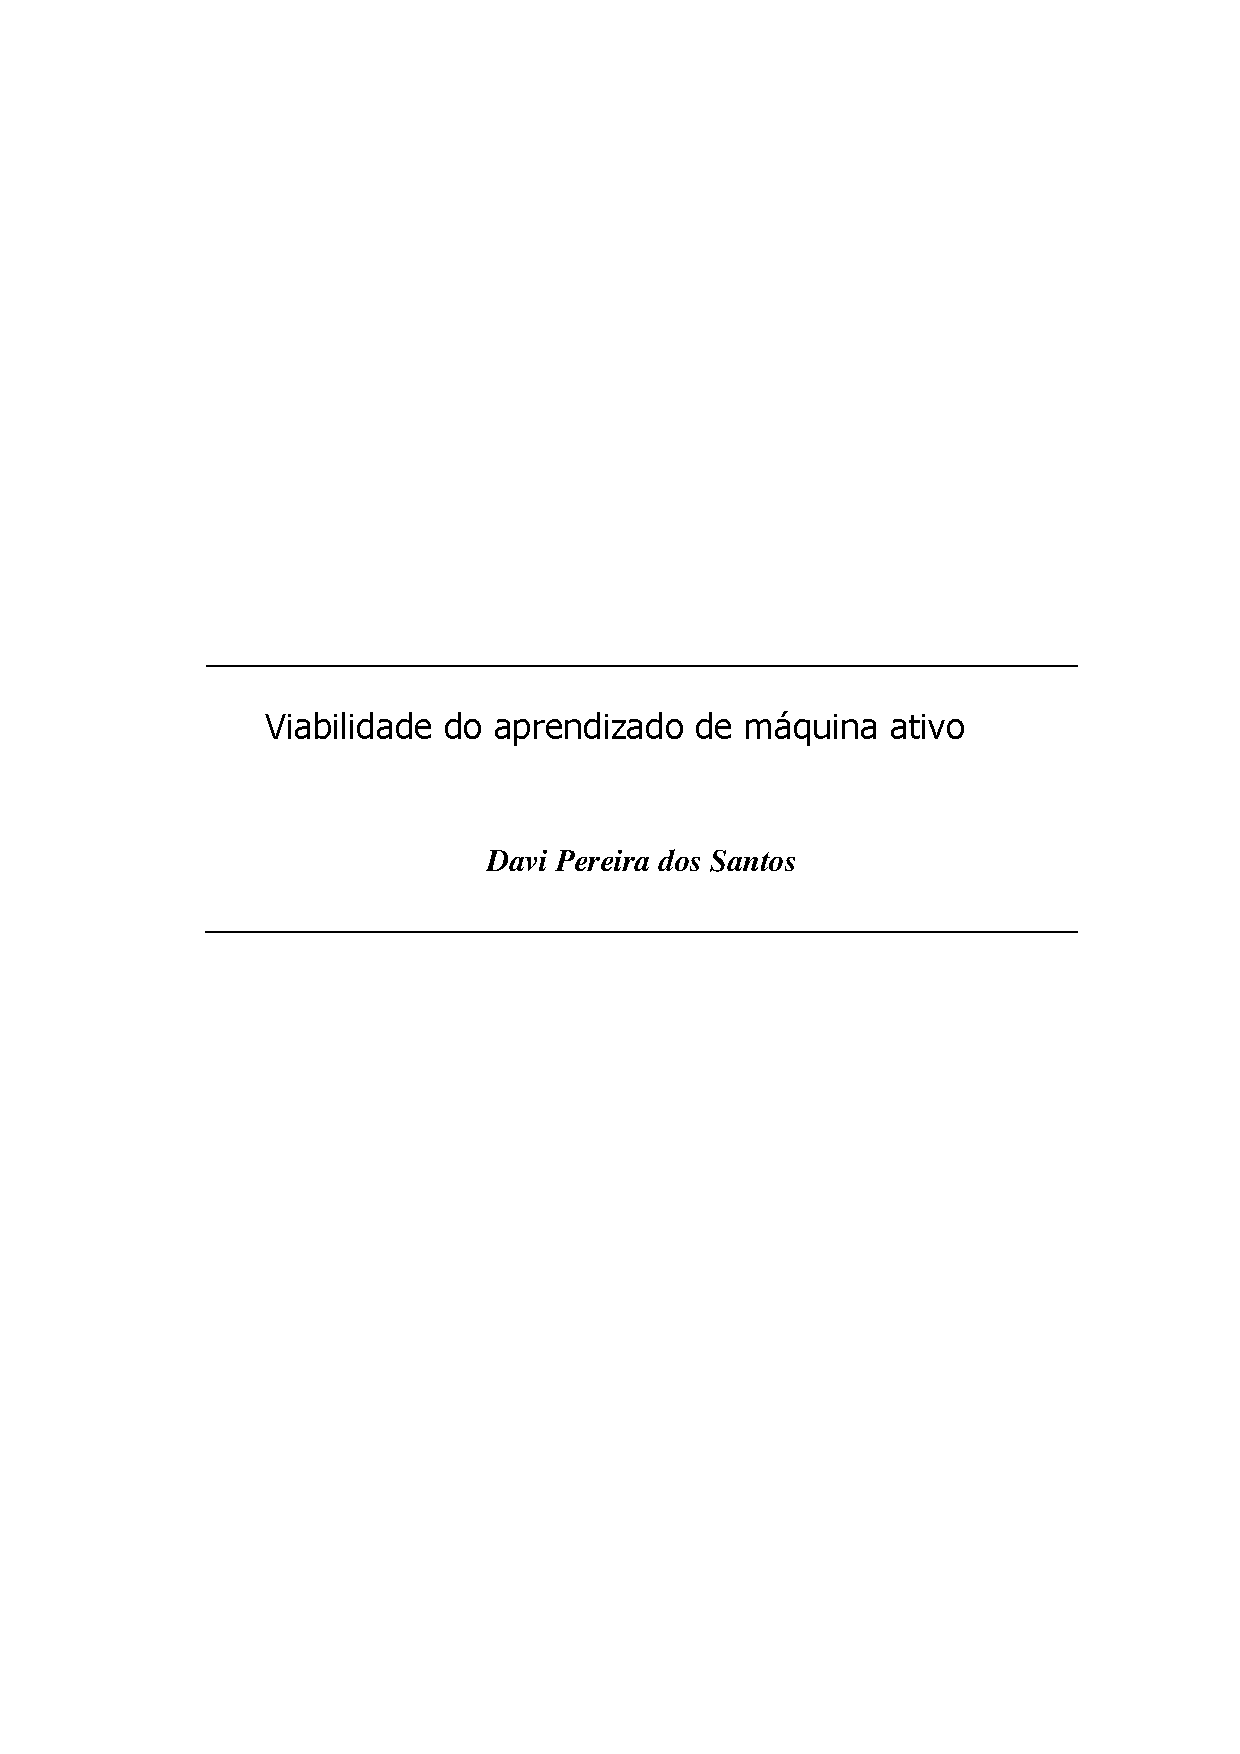
\includepdf[scale=1.06]{SECAO-POSGRAD_87_Modelo_Capa_DO_CCMC_ORIGINAL1.pdf}
  \cleardoublepage
  \newpage
  \clearpage
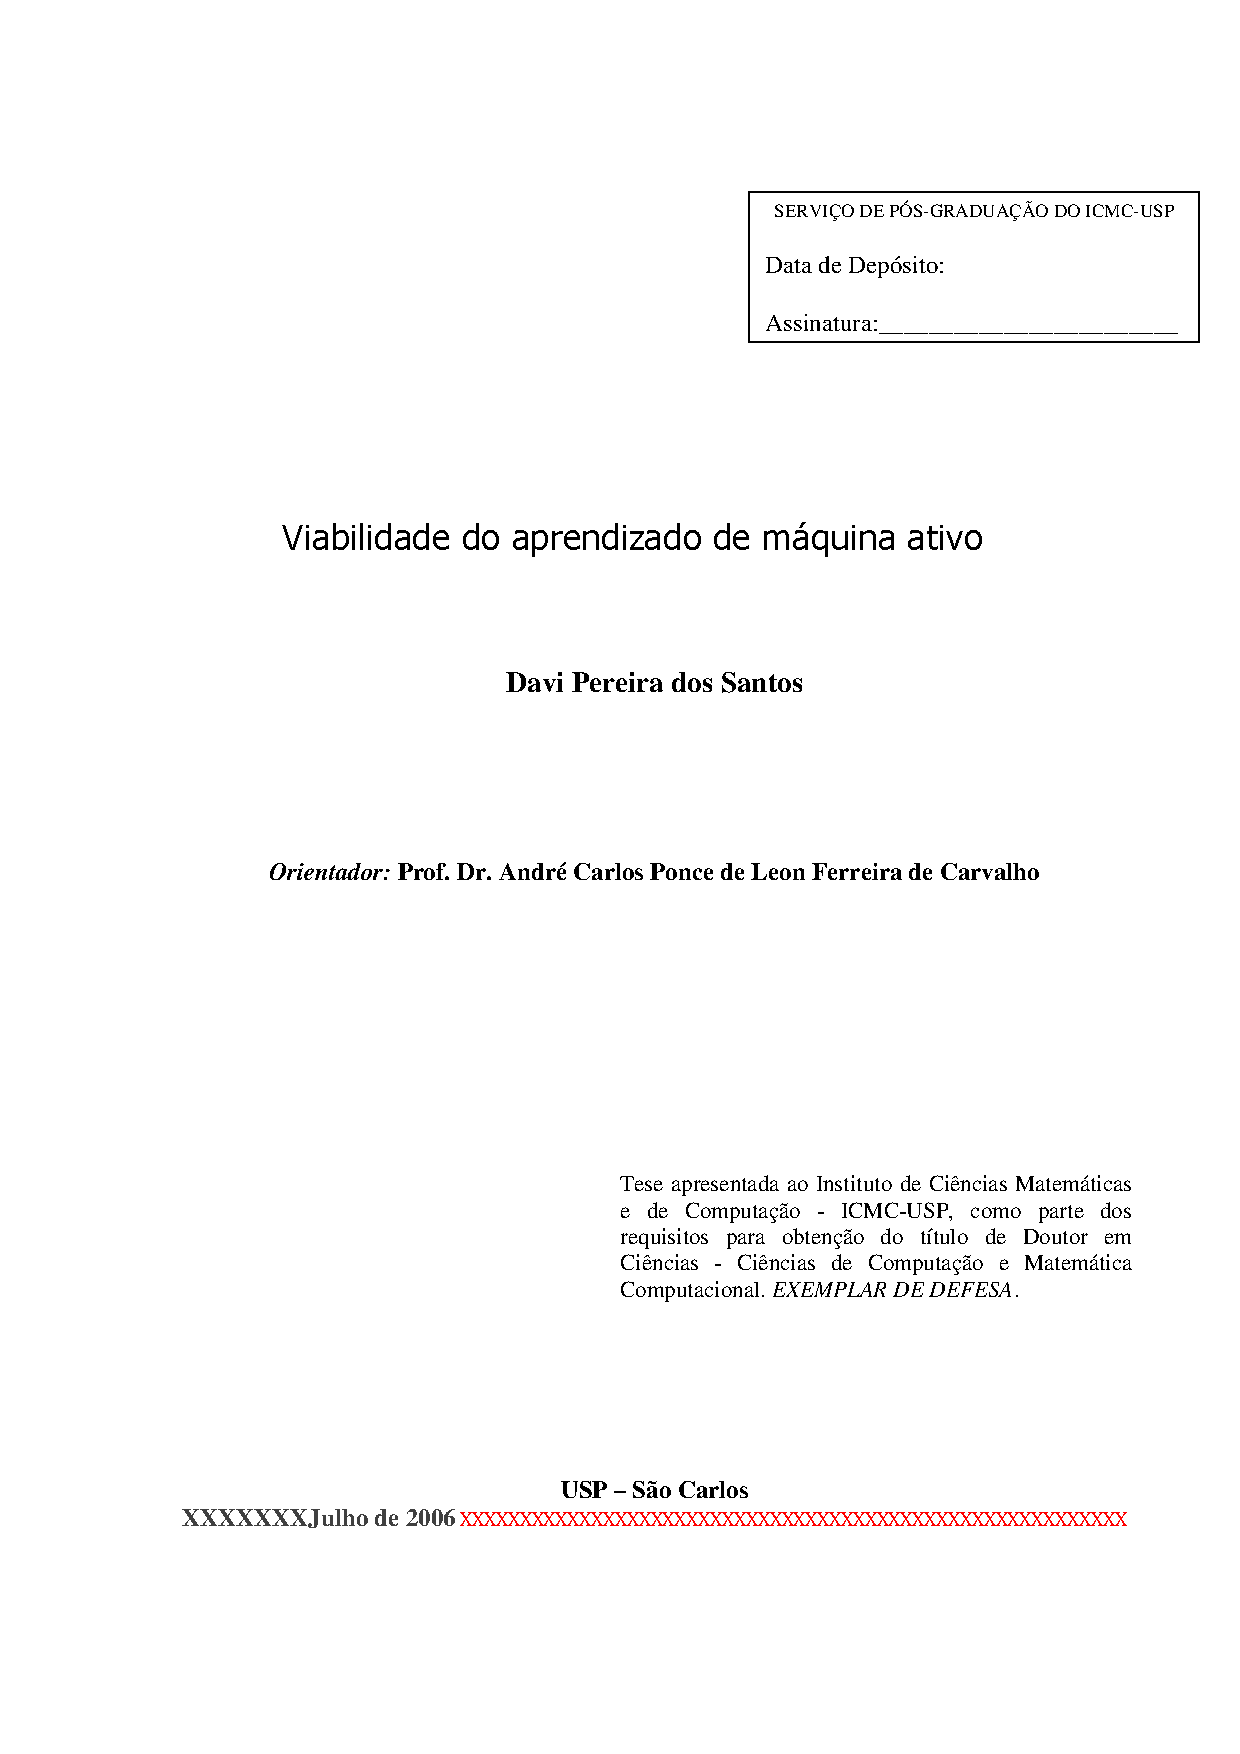
\includepdf[scale=1.06]{SECAO-POSGRAD_87_Modelo_Capa_DO_CCMC_ORIGINAL2.pdf}
\cleardoublepage
\end{titlepage}
\tikzexternalenable
\pagestyle{plain}
\onehalfspacing
\chapter*{Resumo}
Apesar do crescente avan�o no desenvolvimento de algoritmos capazes de induzir modelos preditivos
numa grande diversidade de dom�nios, entraves de cunho econ�mico, dentre outros, ainda persistem.
Embora tais modelos sejam constru�dos sem programa��o expl�cita,
eles n�o podem, em geral, dispensar a supervis�o humana no processo inicial de descoberta de r�tulos que
normalmente se atribuem a certas parcelas dos dados dispon�veis.
Em vista da forte possibilidade dos dados serem massivos,
as parcelas n�o podem ser proporcionais ao total de dados.
Elas devem permanecer pequenas, dentro do devido or�amento.
Isso prop�e um compromisso entre o custo de rotula��o e a acur�cia preditiva,
cuja solu��o pode ser a ado��o de uma t�cnica de aprendizado ativo.

Existem diversas abordagens de se amostrarem ativamente os dados para rotula��o.
Diferentemente do aprendizado passivo, n�o � poss�vel test�-las para posterior escolha da melhor
segundo alguma m�trica de acur�cia.
A cada r�tulo obtido incorre-se em custo adicional.
Dessa forma, a situa��o ideal seria a ci�ncia pr�via da melhor estrat�gia
para o dom�nio em quest�o, mesmo com poucos r�tulos conhecidos de antem�o;
ou, em maior detalhe,
para cada instante durante a aquisi��o de r�tulos naquele dom�nio.

Nesta tese, a viabilidade do aprendizado ativo � comprovada empiricamente com solidez estat�stica 
de acordo com tr�s pontos de vista: adapta��o e compara��o dos principais paradigmas e de sua efetividade em geral;
na defini��o de nichos adequados para cada estrat�gia;
e, na demonstra��o de que � poss�vel definir previamente as estrat�gias mais adequadas,
especialmente se for adotado uma chaveamento ao longo do processo de rotula��o.
� tamb�m empreendida uma an�lise amplamente negligenciada pela literatura da �rea:
o risco devido � variabilidade dos algoritmos.

% o vi�s de amostragem tem seus perigos, ent�o quando n�o h� diferen�a estat�stica entre aleat�rio e AA, deve-se prefirir aleat�rio,
% ou melhor, cluster-based, por suas garantias estatisticas peculiares.

\newpage
\thispagestyle{empty}
\mbox{}
\cleardoublepage

\tableofcontents
\cleardoublepage

\listoffigures
\addcontentsline{toc}{section}{Lista de Figuras}
\cleardoublepage

\listoftables
\addcontentsline{toc}{section}{Lista de Tabelas}
\cleardoublepage

\chapter*{Abreviaturas}
\addcontentsline{toc}{section}{Abreviaturas} %ver comando do rigolin para criar links e outras
\begin{acronym}
\acro{SMOOTE}{Synthetic Minority Over-sampling TEchnique} \acro{QoS }{Quality of Service}
\acro{DDM}{\textit{Drift Detection Method}}
\acro{AWE}{\textit{Drift Detection Method}}
\acro{SEA}{\textit{Streaming Ensemble Algorithm}}
\end{acronym}
\cleardoublepage

\listofalgorithms
\addcontentsline{toc}{section}{Lista de Algoritmos}
\cleardoublepage

\hypersetup{pageanchor=true}
\pagenumbering{arabic}
\pagestyle{fancy}
\renewcommand{\chaptermark}[1]{\markboth{\thechapter \ #1}{}}
\renewcommand{\sectionmark}[1]{\markright{\thesection \ #1}}

%Capitulos
\input introducao
\input contexto
\input propostas
\input metodologia
\input exp-analise
\input exp-elm
\input exp-meta
\input conclusao
\appendix
\input apendice1
\input apendice2
\input apendice3
\input apendice4
\input apendice5
\bibliographystyle{apalike-br}
% \bibliographystyle{abnt-alf}
\bibliography{bibliografia}
\addcontentsline{toc}{chapter}{Refer�ncias Bibliogr�ficas}
\end{document}